\usepackage{hyperref}
\usepackage[utf8]{inputenc}
\usepackage[T2A]{fontenc}
\usepackage[top=5cm,bottom=3cm,right=3cm,left=3cm]{geometry}
\usepackage{graphicx}

\title{Анализ бинарников - Lab3}
\author{Матвей Русаков m.rusakov@innopolis.university SD-03}
\date{Май 2025}

\begin{document}

    \maketitle


    \section{First Task}
        \subsection{Описание программы}

    Программа на C++ принимает аргумент командной строки и сравнивает его с «паролем»,
    который генерируется на лету функцией \texttt{plouf}.
    Если введённый пароль совпадает, выводится сообщение об успехе, иначе — ошибка.

    \subsubsection{Main функция}

    Ниже приведён дизассемблированный вид функции \texttt{main}:

    \begin{verbatim}
    undefined4 main(int param_1, undefined4 *param_2) {
        char *pcVar1;
        bool bVar2;
        ostream *poVar3;
        undefined4 uVar4;
        allocator local_1e;
        allocator local_1d;
        string local_1c[4];
        string local_18[4];
        string local_14[4];
        undefined4 *local_10;

        local_10 = &param_1;
        if (param_1 < 2) {
            pcVar1 = (char *)*param_2;
            poVar3 = std::operator<<((ostream *)std::cerr, "usage : ");
            poVar3 = std::operator<<(poVar3, pcVar1);
            poVar3 = std::operator<<(poVar3, " password");
            std::ostream::operator<<(poVar3, std::endl<>);
            uVar4 = 5;
        }
        else {
            std::allocator<char>::allocator();
            std::string::string(local_14, &DAT_08048dc4, &local_1d);
            std::allocator<char>::allocator();
            std::string::string(local_18, &DAT_08048dcc, &local_1e);
            plouf(local_1c, local_18, local_14);
            std::string::~string(local_18);
            std::allocator<char>::~allocator((allocator<char> *)&local_1e);
            std::string::~string(local_14);
            std::allocator<char>::~allocator((allocator<char> *)&local_1d);
            bVar2 = std::operator==(local_1c, (char *)param_2[1]);
            if (bVar2) {
                poVar3 = std::operator<<((ostream *)std::cout, "Bravo, tu peux valider...");
                std::ostream::operator<<(poVar3, std::endl<>);
            }
            else {
                poVar3 = std::operator<<((ostream *)std::cout, "Password incorrect.");
                std::ostream::operator<<(poVar3, std::endl<>);
            }
            uVar4 = 0;
            std::string::~string(local_1c);
        }
        return uVar4;
    }
    \end{verbatim}

    \subsubsection{Функция \texttt{plouf}}

    Функция \texttt{plouf} принимает три аргумента (результирующую строку, ключ и зашифрованную строку) и применяет поэлементное XOR-сложение между байтами ключа и данных.

    \begin{verbatim}
string *plouf(string *param_1, uint param_2, uint param_3) {
    byte bVar1;
    byte *pbVar2;
    char *pcVar3;
    allocator local_21;
    int local_20;

    std::allocator<char>::allocator();
    std::string::string(param_1, "", &local_21);
    std::allocator<char>::~allocator((allocator<char> *)&local_21);
    local_20 = 0;
    while (true) {
        pcVar3 = (char *)std::string::operator[](param_2);
        if (*pcVar3 == '\0') break;
        pbVar2 = (byte *)std::string::operator[](param_2);
        bVar1 = *pbVar2;
        std::string::length();
        pbVar2 = (byte *)std::string::operator[](param_3);
        std::string::operator+=(param_1, *pbVar2 ^ bVar1);
        local_20 = local_20 + 1;
    }
    return param_1;
}
    \end{verbatim}

    \subsection{Данные}

    В памяти были обнаружены два массива байтов:

    \begin{itemize}
        \item Ключ (\texttt{DAT\_08048dc4}):
        \[
            18 \; D6 \; 15 \; CA \; FA \; 77 \; 00
        \]
        \item Зашифрованные данные (\texttt{DAT\_08048dcc}):

        50 \; B3 \; 67 \; AF \; A5 \; 0E \; и так далее (будет в питон скрипте)

    \end{itemize}

    Важно: последний байт ключа (\texttt{00}) — это нулевой символ конца строки, используемый C++ для терминации строки,
    и \textbf{не участвует в шифровании}.

    \subsection{Процесс дешифрования}

    Алгоритм дешифрования прост: каждый байт зашифрованной строки XOR-ится с очередным байтом ключа,
    ключ повторяется циклически каждые 6 байт.

    Python-скрипт для расшифровки:

    \begin{verbatim}
        key = [0x18, 0xD6, 0x15, 0xCA, 0xFA, 0x77]  # 6 байт, без \0
        encrypted = [
            0x50,0xB3,0x67,0xAF,0xA5,0x0E,0x77,0xA3,0x4A,0xA2,
            0x9B,0x01,0x7D,0x89,0x61,0xA5,0xA5,0x02,0x76,0xB2,
            0x70,0xB8,0x89,0x03,0x79,0xB8,0x71,0x95,0x9B,0x28,
            0x74,0xBF,0x61,0xBE,0x96,0x12,0x47,0x95,0x3E,0xE1,
            0xA5,0x04,0x6C,0xA3,0x73,0xAC,0x89,0x00
        ]

        decrypted = ""
        for i in range(len(encrypted)):
            decrypted += chr(encrypted[i] ^ key[i % len(key)])

        print(decrypted)
    \end{verbatim}

    \subsection{Результат}

    Выход скрипта:

    \begin{quote}
        Here\_you\_have\_to\_understand\_a\_little\_C++\_stuffs
    \end{quote}
    Что и является паролем, на мой взгляд

    \subsection{Тестовые запуски}

    \paragraph{}
    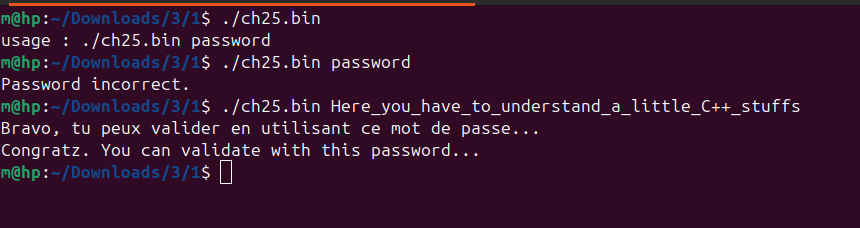
\includegraphics[width=1\linewidth]{static/solution_1}


    \section{Second Task}
        \subsection{Main функция}

    \begin{verbatim}
        undefined4 main(void)

        {
          char *pcVar1;
          int iVar2;
          undefined4 local_10;

          puts("############################################ ################");
          puts("##        Bienvennue dans ce challenge de cracking        ##" );
          puts("############################################ ################\n");
          printf("username: ");
          pcVar1 = (char *)getString(local_10);
          iVar2 = strcmp(pcVar1,"john");
          if (iVar2 == 0) {
             printf("password: ");
             pcVar1 = (char *)getString(pcVar1);
             iVar2 = strcmp(pcVar1,"the ripper");
             if (iVar2 == 0) {
                printf("Bien joue, vous pouvez valider l'epreuve avec le mot d e passe : %s !\n","987654321");
             }
             else {
                puts("Bad password");
             }
          }
          else {
             puts("Bad username");
          }
          return 0;
        }
    \end{verbatim}

    \subsection{Описание}

    Программа реализует простую аутентификационную логику.
    Пользователю предлагается ввести имя пользователя и пароль.
    Проверка осуществляется путём прямого сравнения введённых строк с жёстко заданными значениями.

    \begin{itemize}
        \item Если имя пользователя совпадает с \texttt{"john"}, то далее проверяется пароль.
        \item Если пароль совпадает с \texttt{"the ripper"}, то выводится сообщение об успехе и секретный ключ.
        \item В противном случае программа сообщает об ошибке (\texttt{"Bad username"} или \texttt{"Bad password"}).
    \end{itemize}

    \subsection*{Ключ (флаг)}

    Если логин и пароль указаны верно, программа выводит:

    \begin{verbatim}
        Bien joue, vous pouvez valider l'epreuve avec le mot de passe : 987654321 !
    \end{verbatim}


    \subsection{Особенности}

    \begin{itemize}
        \item Логика крайне простая — всё полностью зашито в бинарник.
        \item Пароли не шифруются, не хэшируются и не скрыты — можно легко найти через \texttt{strings} или дизассемблирование.
        \item Юзернейм - "john", пароль - "the ripper"
        \item Ключ - 987654321
    \end{itemize}

    \subsection{Тестовые запуски}
    \paragraph{}
    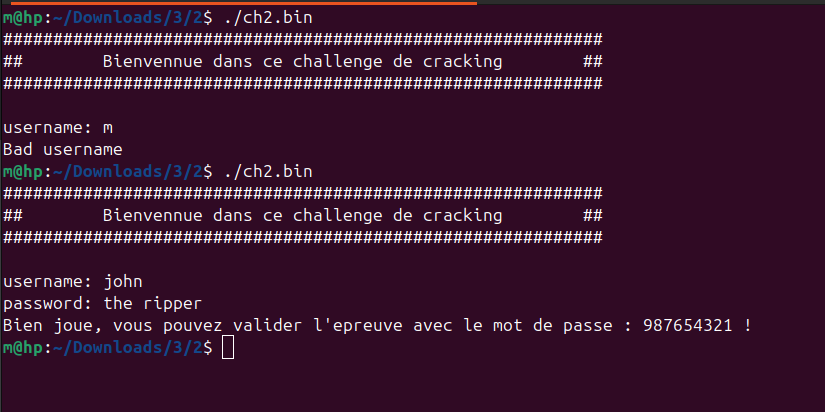
\includegraphics[width=1\linewidth]{static/solution_2}


    \begin{thebibliography}{1}
        \bibitem{githublink}
        GitHub Link: https://github.com/MattWay224/reverse-engineering-course
        В этом репозитории можно найти все лабы и информацию про каждое задание в каждой лабе
    \end{thebibliography}
\end{document}
